\section*{11 березня 2019 р.}

\setcounter{problem}{0}

\begin{problem}
    Розв'язати задачу багато-критеріальної оптимізації \[ f_1 = - x_1 - x_2 \to \max, \quad f_2 = 2 x_1 + x_2 \to \max, \quad f_3 = x_1 + 3 x_2 \to \max \] з допустимою областю що визначається нерівностями \[ x_1 + x_2 \le 4, \quad x_1 + 2 x_2 \le 6, \quad x_{1, 2} \ge 0 \] методом послідовних поступок (величини поступок вибрати самостійно).
\end{problem}

\begin{solution}
    Перш за все зобразимо допустиму область $G_0$:
    \begin{figure}[H]
        \centering
        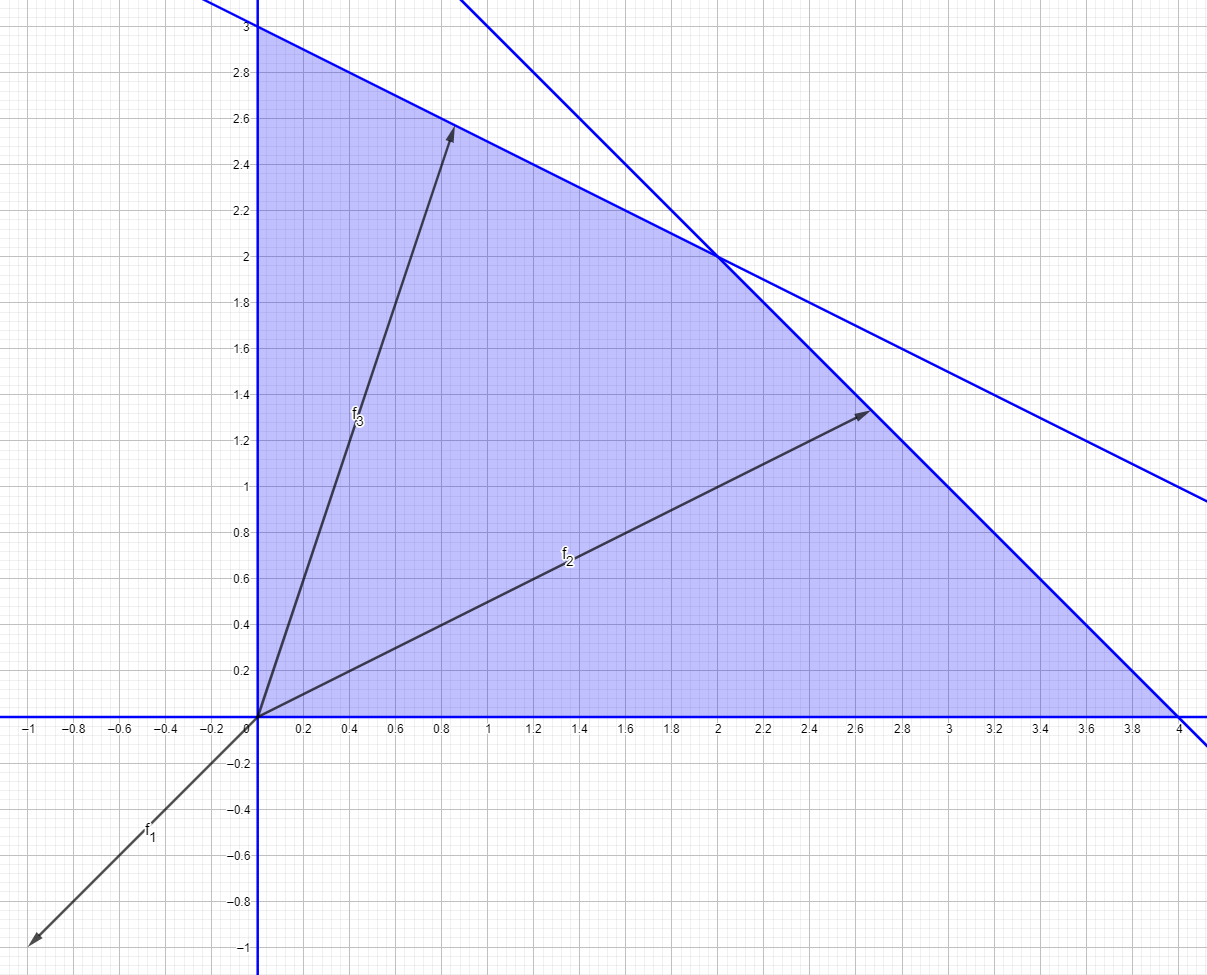
\includegraphics[width=\textwidth]{img/successive_concessions_1_1.png}
    \end{figure}

    З графічних міркувань знаходимо \[ \tilde x_1 = \arg \max f_1(x_1, x_2) = (0, 0), \quad f_1^\star = \max_{x \in G_0} f_1(x_1, x_2) = 0. \]
    
    Покладаючи величину поступки $\Delta f_1$ за першим критерієм рівною $2$ отримуємо, що до допустимої області додається умова \[ f_1(x_1, x_2) \ge f_1^\star - \Delta f_1 = -2, \] тому уточнена допустима область $G_1$ має вигляд:
    \begin{figure}[H]
        \centering
        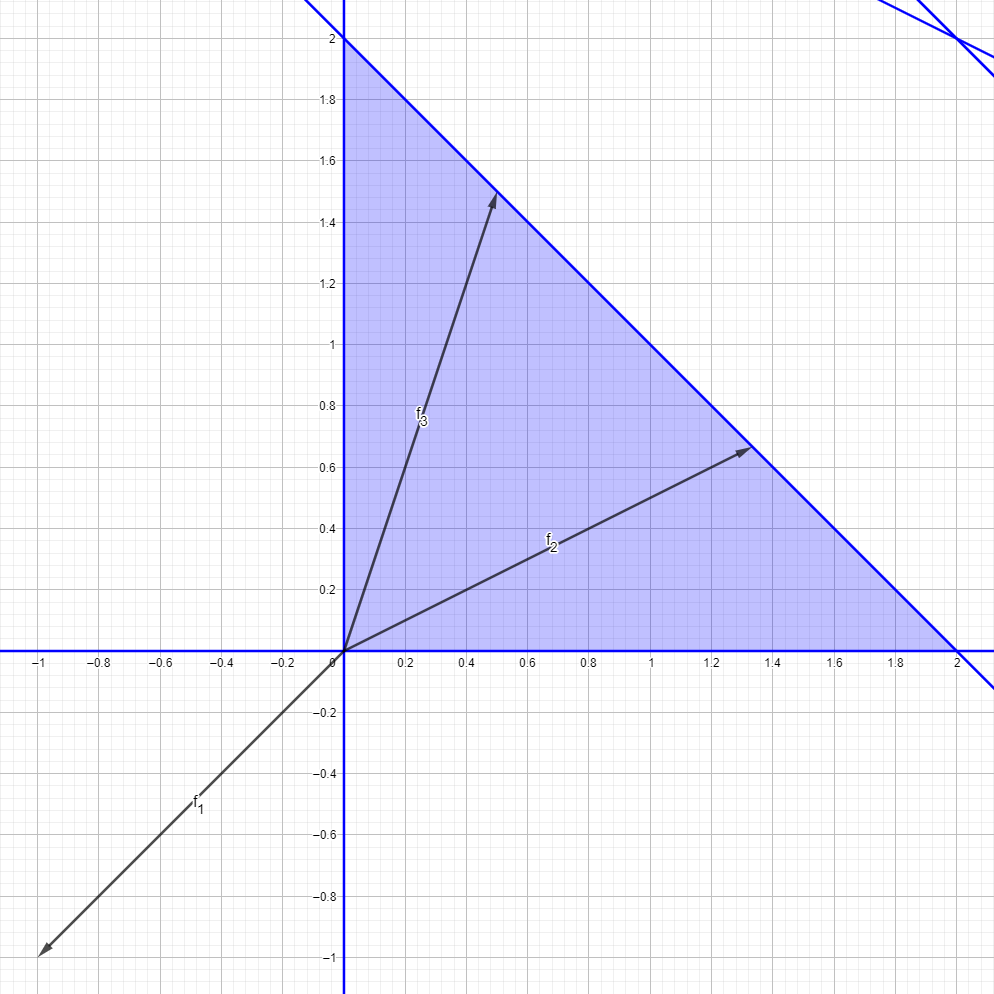
\includegraphics[width=\textwidth]{img/successive_concessions_1_2.png}
    \end{figure}

    З графічних міркувань знаходимо \[ \tilde x_2 = \arg \max f_2(x_1, x_2) = (2, 0), \quad f_2^\star = \max_{x \in G_1} f_2(x_1, x_2) = 4. \]
    
    Покладаючи величину поступки $\Delta f_2$ за другим критерієм рівною $2$ отримуємо, що до допустимої області додається умова \[ f_2(x_1, x_2) \ge f_2^\star - \Delta f_2 = 2, \] тому уточнена допустима область $G_2$ має вигляд:
    \begin{figure}[H]
        \centering
        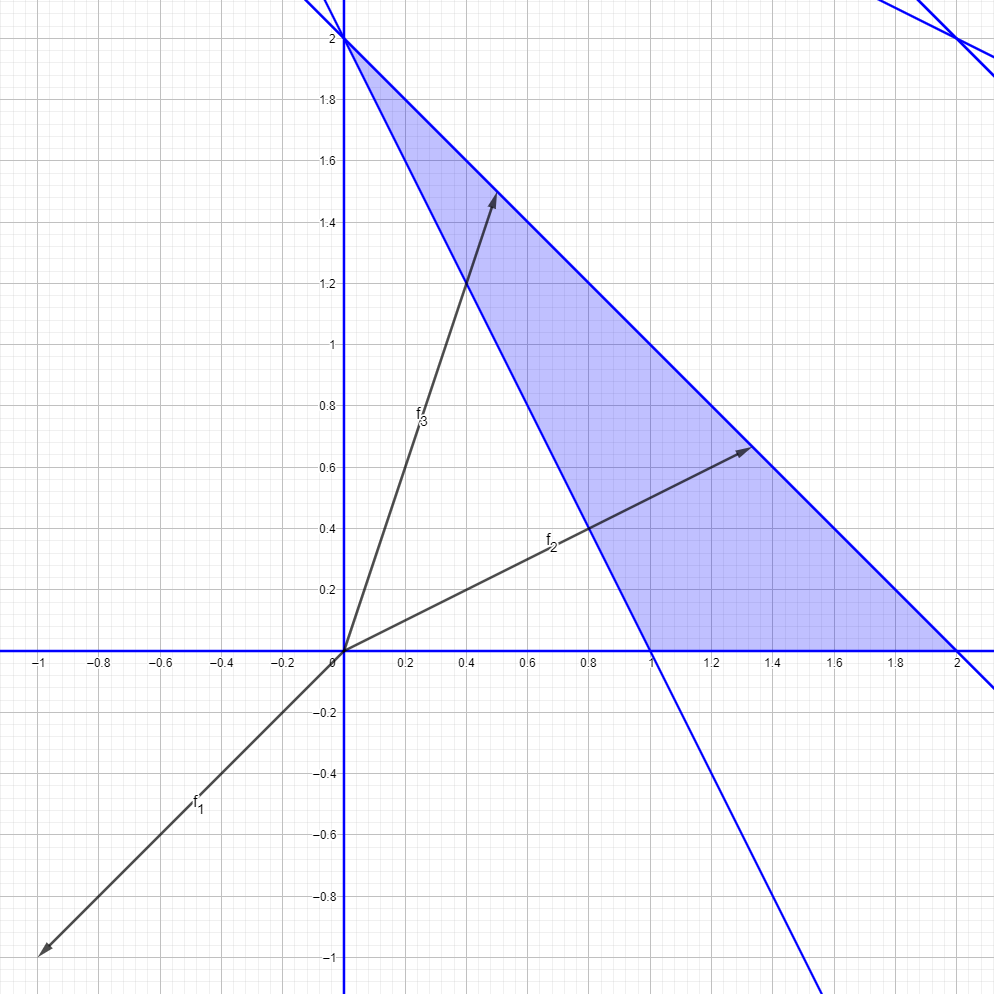
\includegraphics[width=\textwidth]{img/successive_concessions_1_3.png}
    \end{figure}

    З графічних міркувань знаходимо \[ \tilde x_3 = \arg \max f_3(x_1, x_2) = (0, 2), \quad f_3^\star = \max_{x \in G_2} f_3(x_1, x_2) = 6. \]
    
    Оскільки це останній критерій, то ми не робимо поступок, а просто кажемо, що знайдена точка $\tilde x_3$ є розв'язком $x^\star$. \medskip
    
    Наостанок зауважимо, що $f(x^\star) = (-2, 2, 6)$.
\end{solution}

\newpage

\begin{problem}
    Розв'язати задачу багато-критеріальної оптимізації \[ f_1 = - x_1 - 2 x_2 \to \max, \quad f_2 = 2 x_1 + x_2 \to \max, \quad f_3 = x_1 + 3 x_2 \to \max \] з допустимою областю що визначається нерівностями \[ x_1 + x_2 \le 4, \quad 2 x_1 + x_2 \le 6, \quad x_{1, 2} \ge 0 \] методом послідовних поступок (величини поступок вибрати самостійно).
\end{problem}

\begin{solution}
    Перш за все зобразимо допустиму область $G_0$:
    \begin{figure}[H]
        \centering
        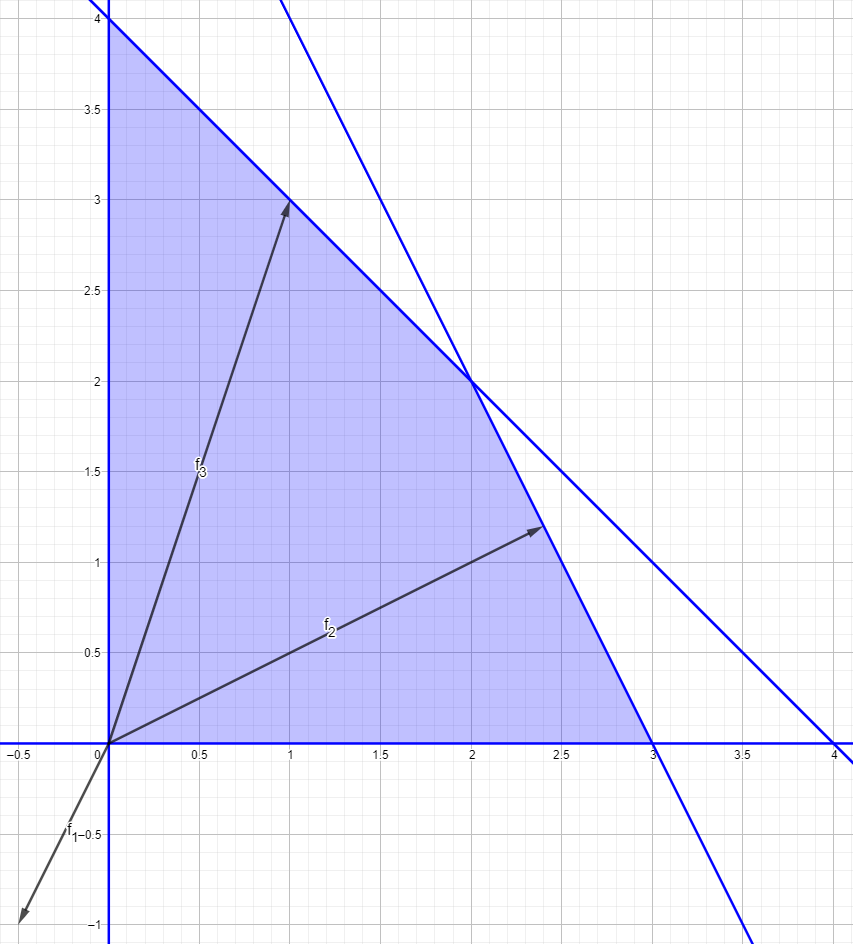
\includegraphics[width=\textwidth]{img/successive_concessions_2_1.png}
    \end{figure}

    З графічних міркувань знаходимо \[ \tilde x_1 = \arg \max f_1(x_1, x_2) = (0, 0), \quad f_1^\star = \max_{x \in G_0} f_1(x_1, x_2) = 0. \]
    
    Покладаючи величину поступки $\Delta f_1$ за першим критерієм рівною $4$ отримуємо, що до допустимої області додається умова \[ f_1(x_1, x_2) \ge f_1^\star - \Delta f_1 = -4, \] тому уточнена допустима область $G_1$ має вигляд:
    \begin{figure}[H]
        \centering
        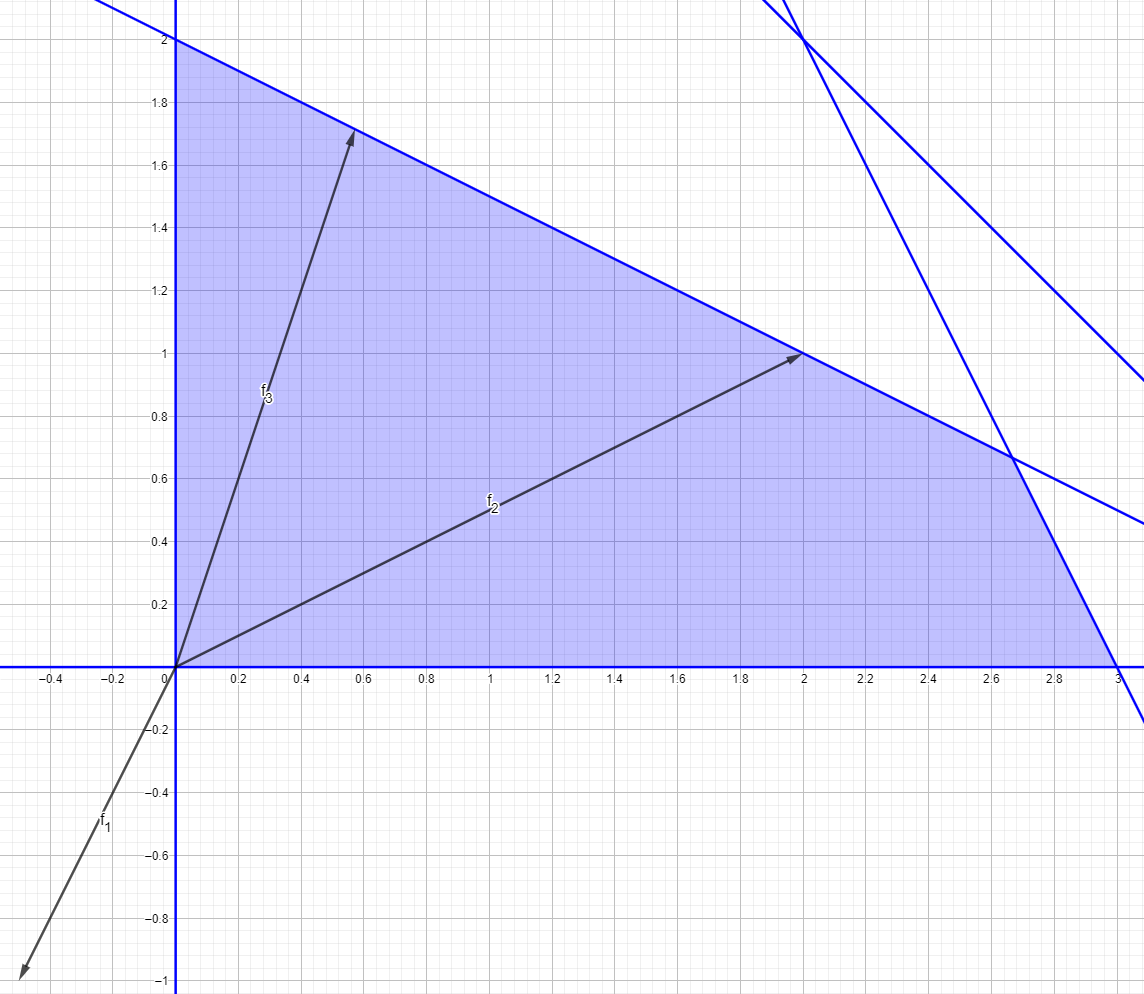
\includegraphics[width=\textwidth]{img/successive_concessions_2_2.png}
    \end{figure}

    З графічних міркувань знаходимо \[ \tilde x_2 = \arg \max f_2(x_1, x_2) = (3 - t, 2 t), \ t \in \left[0, \frac13\right], \quad f_2^\star = \max_{x \in G_1} f_2(x_1, x_2) = 6. \]

    Покладаючи величину поступки $\Delta f_2$ за другим критерієм рівною $3$ отримуємо, що до допустимої області додається умова \[ f_2(x_1, x_2) \ge f_2^\star - \Delta f_2 = 3, \] тому уточнена допустима область $G_2$ має вигляд:
    \begin{figure}[H]
        \centering
        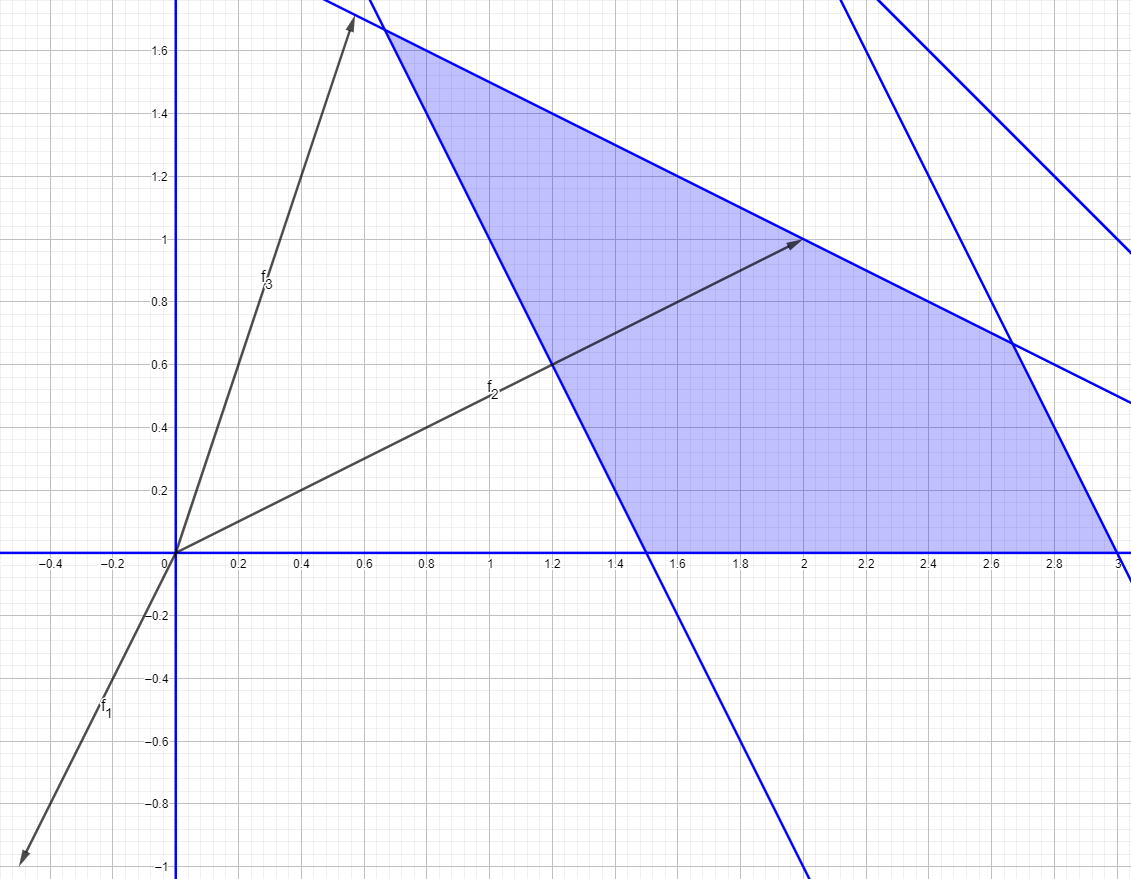
\includegraphics[width=\textwidth]{img/successive_concessions_2_3.png}
    \end{figure}

    З графічних міркувань знаходимо \[ \tilde x_3 = \arg \max f_3(x_1, x_2) = \left(\frac23, 1\ \frac23\right), \quad f_3^\star = \max_{x \in G_2} f_3(x_1, x_2) = 5\ \frac23. \]
    
    Оскільки це останній критерій, то ми не робимо поступок, а просто кажемо, що знайдена точка $\tilde x_3$ є розв'язком $x^\star$. \medskip
    
    Наостанок зауважимо, що \[ f(x^\star) = \left(-4, 3, 5\ \frac23\right).\]
\end{solution}

\newpage